\documentclass[abstract=on,9pt,twocolumn]{scrartcl}

\usepackage{ucs}
\usepackage[utf8x]{inputenc}
\usepackage[T1]{fontenc}
\usepackage[english]{babel}
\usepackage{datetime}
%\usepackage{multicol}
\usepackage{float}

\usepackage[paper=a4paper,top=2cm,left=1.5cm,right=1.5cm,bottom=2cm,foot=1cm]{geometry}

\usepackage{relsize}%	relative font sizes

\usepackage[retainorgcmds]{IEEEtrantools}%	IEEEeqnarray
\setlength{\IEEEnormaljot}{4\IEEEnormaljot}

\usepackage{graphicx}
\usepackage{epstopdf}
\usepackage{indentfirst}
\usepackage[hyphens]{url}
\usepackage[linktocpage]{hyperref}
%\usepackage{hyperref}
%\usepackage{cleveref}
\usepackage[noabbrev]{cleveref}
\usepackage{listings}
\usepackage{color}
\usepackage{subfig}

%%%%%%%%%%%%%%%%
%  title page  %
%%%%%%%%%%%%%%%%
\titlehead{University of Texas at Austin \hfill Institute for Computational Engineering and Sciences (ICES)}
\title{GMetis - Xeon Phi}

\author{
    \\David Pereira\\
     	\texttt{\smaller pg22821@alunos.uminho.pt}
\\~\\~
\and\\Rui Brito\\
	\texttt{\smaller pg22781@alunos.uminho.pt}
}

\date{Austin, \docdate}

%%%%%%%%%%%
%  Hacks  %
%%%%%%%%%%%

%	Paragraph (title) with linebreak
\newcommand{\paragraphh}[1]{\paragraph{#1\hfill}\hfill

}

%	Add "Appendix" to the appendices titles, but not to the references
\usepackage{ifthen}
\newcommand*{\appendixmore}{%
  \renewcommand*{\othersectionlevelsformat}[1]{%
    \ifthenelse{\equal{##1}{section}}{\appendixname~}{}%
    \csname the##1\endcsname\autodot\enskip}
  \renewcommand*{\sectionmarkformat}{%
    \appendixname~\thesection\autodot\enskip}
}

\newdateformat{mmmyyyydate}{\monthname[\THEMONTH] \THEYEAR}
\newcommand{\docdate}{\mmmyyyydate\today}


%-----------------------------------------------------------------------------
% Bibliografias usadas e por usar
%-----------------------------------------------------------------------------

%Usadas
%Karypis95parallelmultilevel
%Karypis:1998:FHQ:305219.305248
%Cepeda:PhiPerformance

%Por usar


%-----------------------------------------------------------------------------
% Begin Document
%-----------------------------------------------------------------------------

\begin{document}
\maketitle	


%-----------------------------------------------------------------------------
% Abstract
%-----------------------------------------------------------------------------

\begin{abstract}
In this report, we address GMetis, a graph partitioning application that
uses the Metis algorithm. This application uses the Galois framework
and has as objective reducing the total edgecut of a graph and improving
load balance between partitions. We show scalability measurements of the
application when running it in the brand new Xeon Phi, the first
co-processor from the MIC architecture. We also show some modifications
done in order to reduce the application's runtime. At last, we compare
GMetis with metis and mt-metis, a parallel version of metis which uses
OpenMP, both in terms of runtime and edgecut.
\end{abstract}


%-----------------------------------------------------------------------------
% Introduction
%-----------------------------------------------------------------------------

\section{Introduction}
Metis is actually the most famous graph partitioning algorithm. It was
developed by George
Karypis\footnote{http://glaros.dtc.umn.edu/gkhome/metis/metis/overview}
and the University of Minnesota, and it has as objective to group
weighted graph nodes into partitions so that all partitions have similar
weight (balanced partitions) and to reduce total edgecut, which is the
total weight of all edges between partitions. This algorithm has three
major phases: Coarsening, Partitioning and Refinement.
All phases of this algorithm are explained in
section~\ref{sec:metis_alg}.

The application addressed in this report is \textit{GMetis}, an
application that uses the metis algorithm together with the
\textit{Galois} framework to produce an efficient parallel version of
\textit{Metis}. Our goal was to port GMetis for the Xeon Phi
architecture, optimizing its performance, identifying its
limitations and bottlenecks, and compare its runtime and edgecut with
Metis and its parallel version, mt-metis.

The rest of this report is structured as follows:\\
The Xeon Phi architecture and features are explained in section~\ref{sec:sys_char}.
while section~\ref{sec:enhan} details results and some enhancements made
to improve performance on the Xeon Phi. Section \ref{sec:conc} presents
our final conclusions.


%-----------------------------------------------------------------------------
% Metis Algorithm Description
%-----------------------------------------------------------------------------

\section{The Metis Algorithm}
\label{sec:metis_alg}

  Formally, the metis algorithm consists of three phases. They are as follows:

  \begin{itemize}
  \item Given a graph $G_0 = (V_0,E_0)$:
  \begin{itemize}    
    \item Coarsening:
    \begin{itemize}
      \item $G_0$ is transformed into a sequence of smaller graphs $G_1,G_2,\cdots,G_m$ such that $|V_0|>|V_1|>|V_2|>\cdots>|V_m|$
    \end{itemize}
    \item Partitioning: 
    \begin{itemize}
      \item A 2-way partition $P_m$ of the graph $G_m = (V_m,E_m)$ is computed that partitions $V_m$ into two parts, each containing half the vertices of $G_0$
    \end{itemize}
    \item Refinement:
    \begin{itemize}
      \item The partition $P_m$ of $G_m$ is projected back to $G_0$ by going through intermediate partitions $P_{m-1}, P_{m-2},\cdots,P_1,P_0$
    \end{itemize}
  \end{itemize}
\end{itemize}

Visually, this translates into the following scenarios:

\begin{center}
  \begin{figure}[htb]
    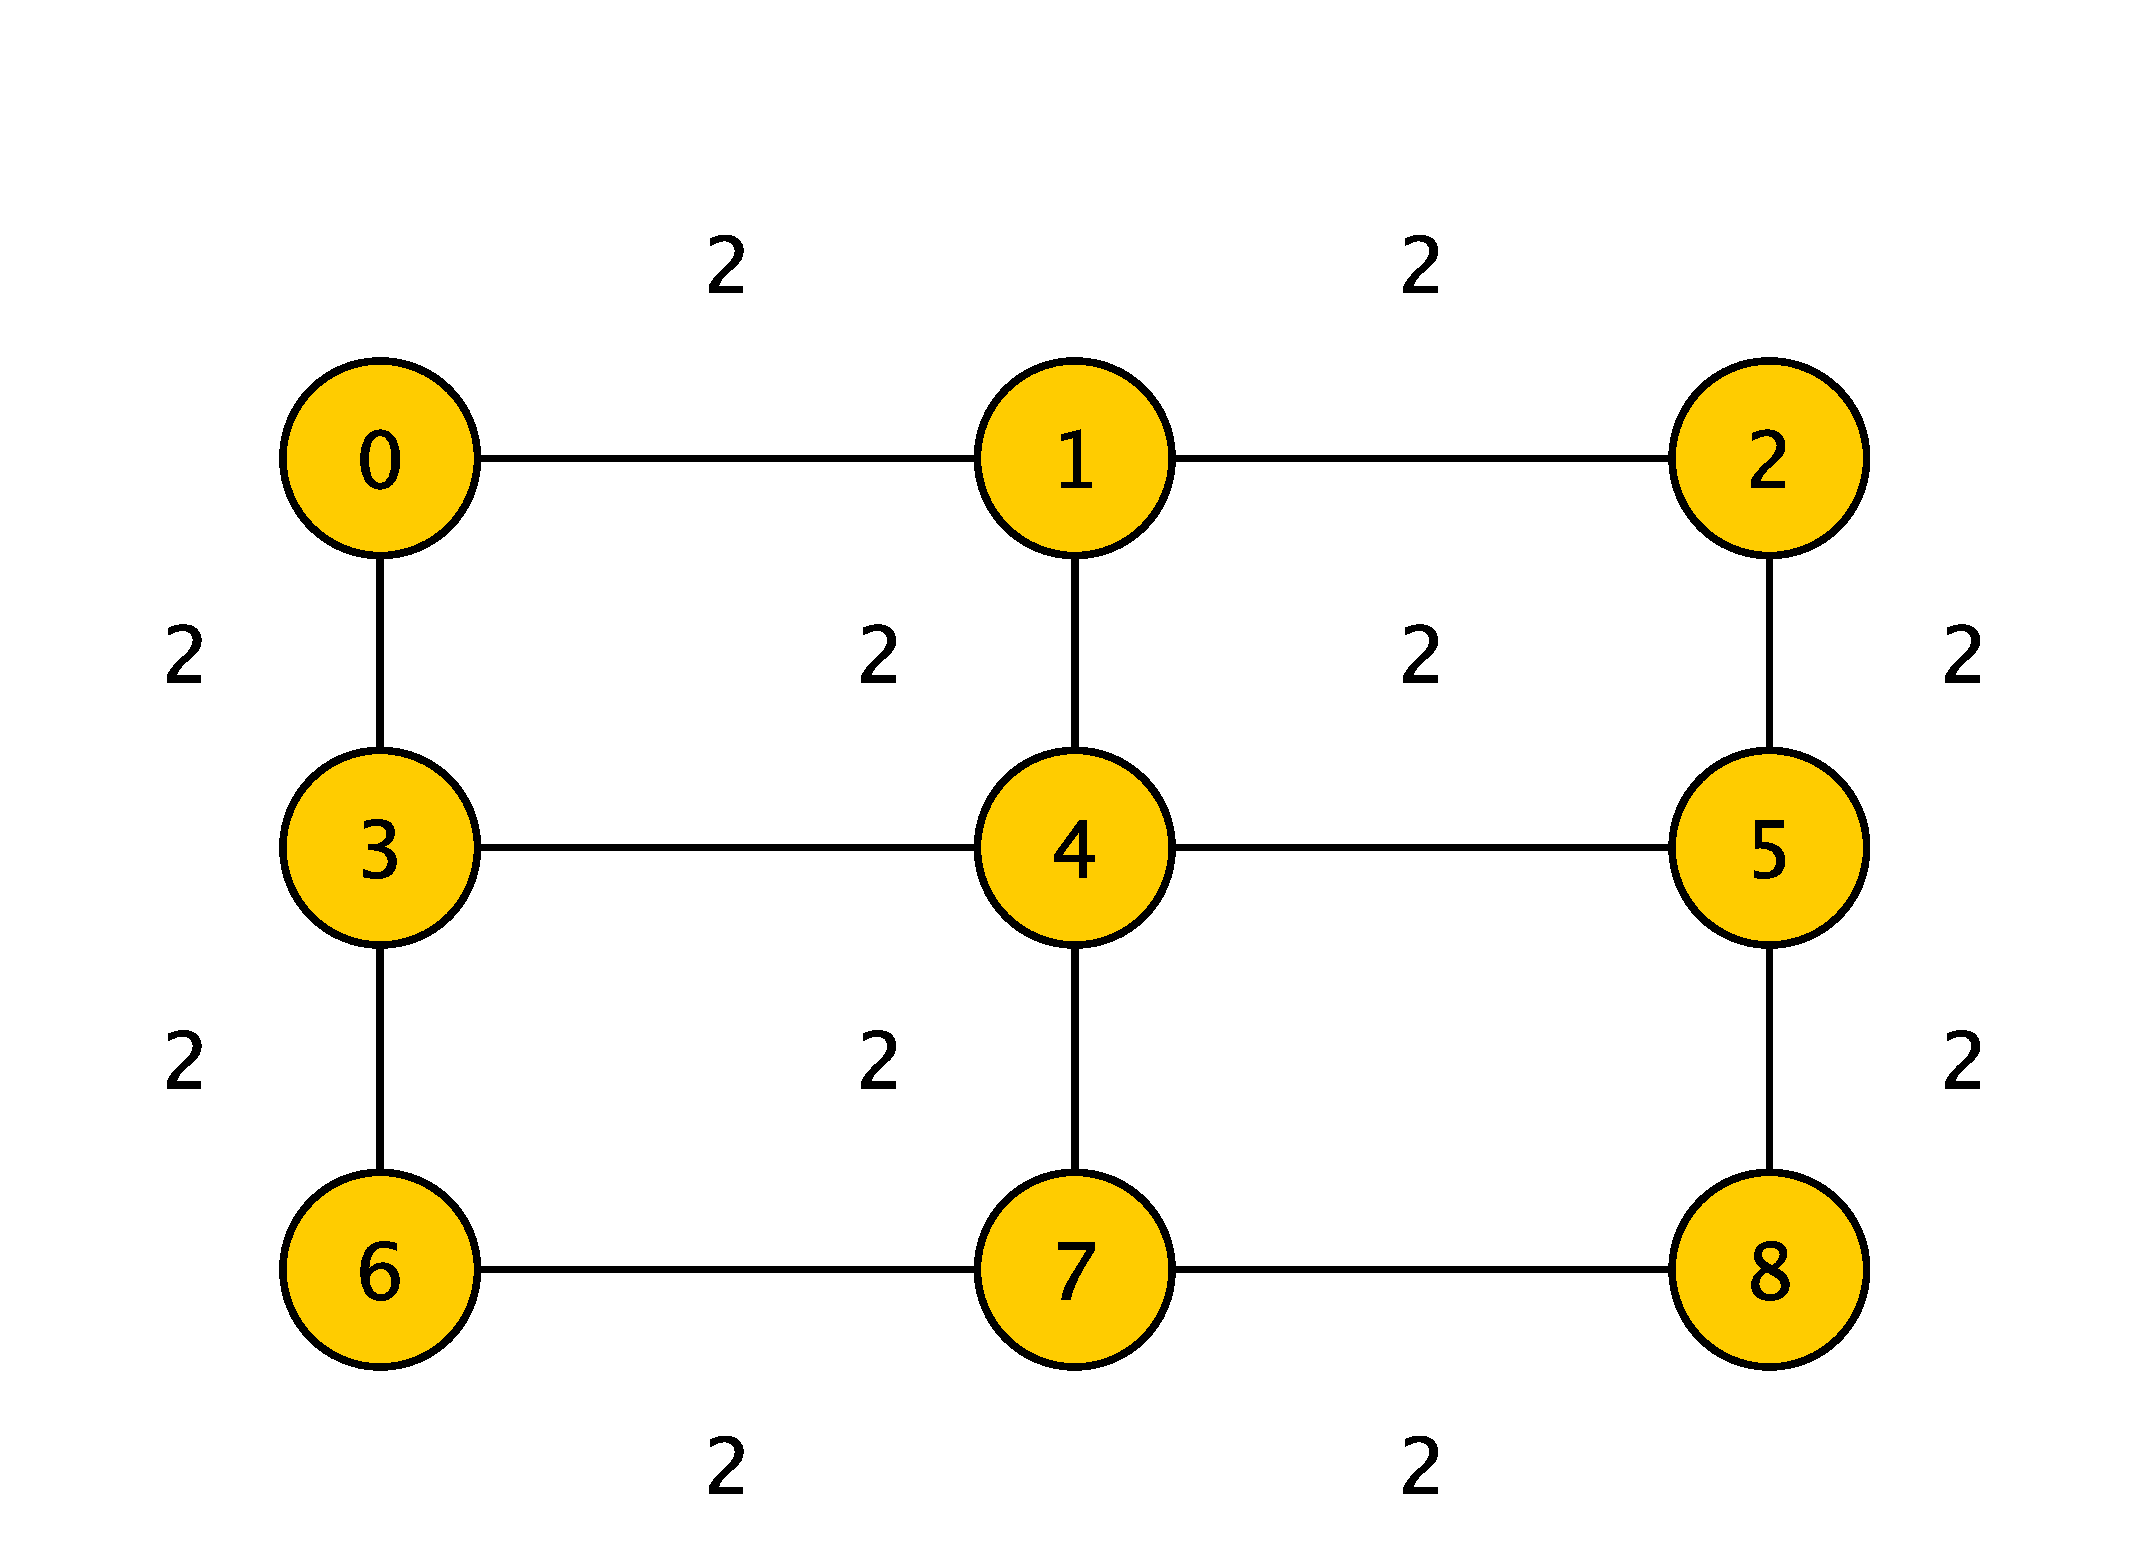
\includegraphics[width=\columnwidth]{img/coarsening.eps}
    \caption{Initial graph}
    \label{img:init_graph}
  \end{figure} 
\end{center}

Figures \ref{img:init_graph} and \ref{img:coarse_graph} illustrate the coarsening phase. During this phase, a sequence of coarser graphs is constructed.\cite{Karypis95parallelmultilevel} A coarser graph is constructed by matching neighbour vertices and then contracting the edges. Thus, the edge between two vertices is collapsed and a multinode consisting of those two vertices is created. Also, the edge-cut of a partition in a coarser graph should be equal to the edge-cut of the same partition in the finer graph.\cite{Karypis:1998:FHQ:305219.305248} This process is achieved in one of two approaches. The first approach consists on finding a random matching and created a multinode with the process described above, while the second approach consists of matching groups of vertices that are highly connected.\cite{Karypis:1998:FHQ:305219.305248}

\begin{center}
  \begin{figure}[htb]
    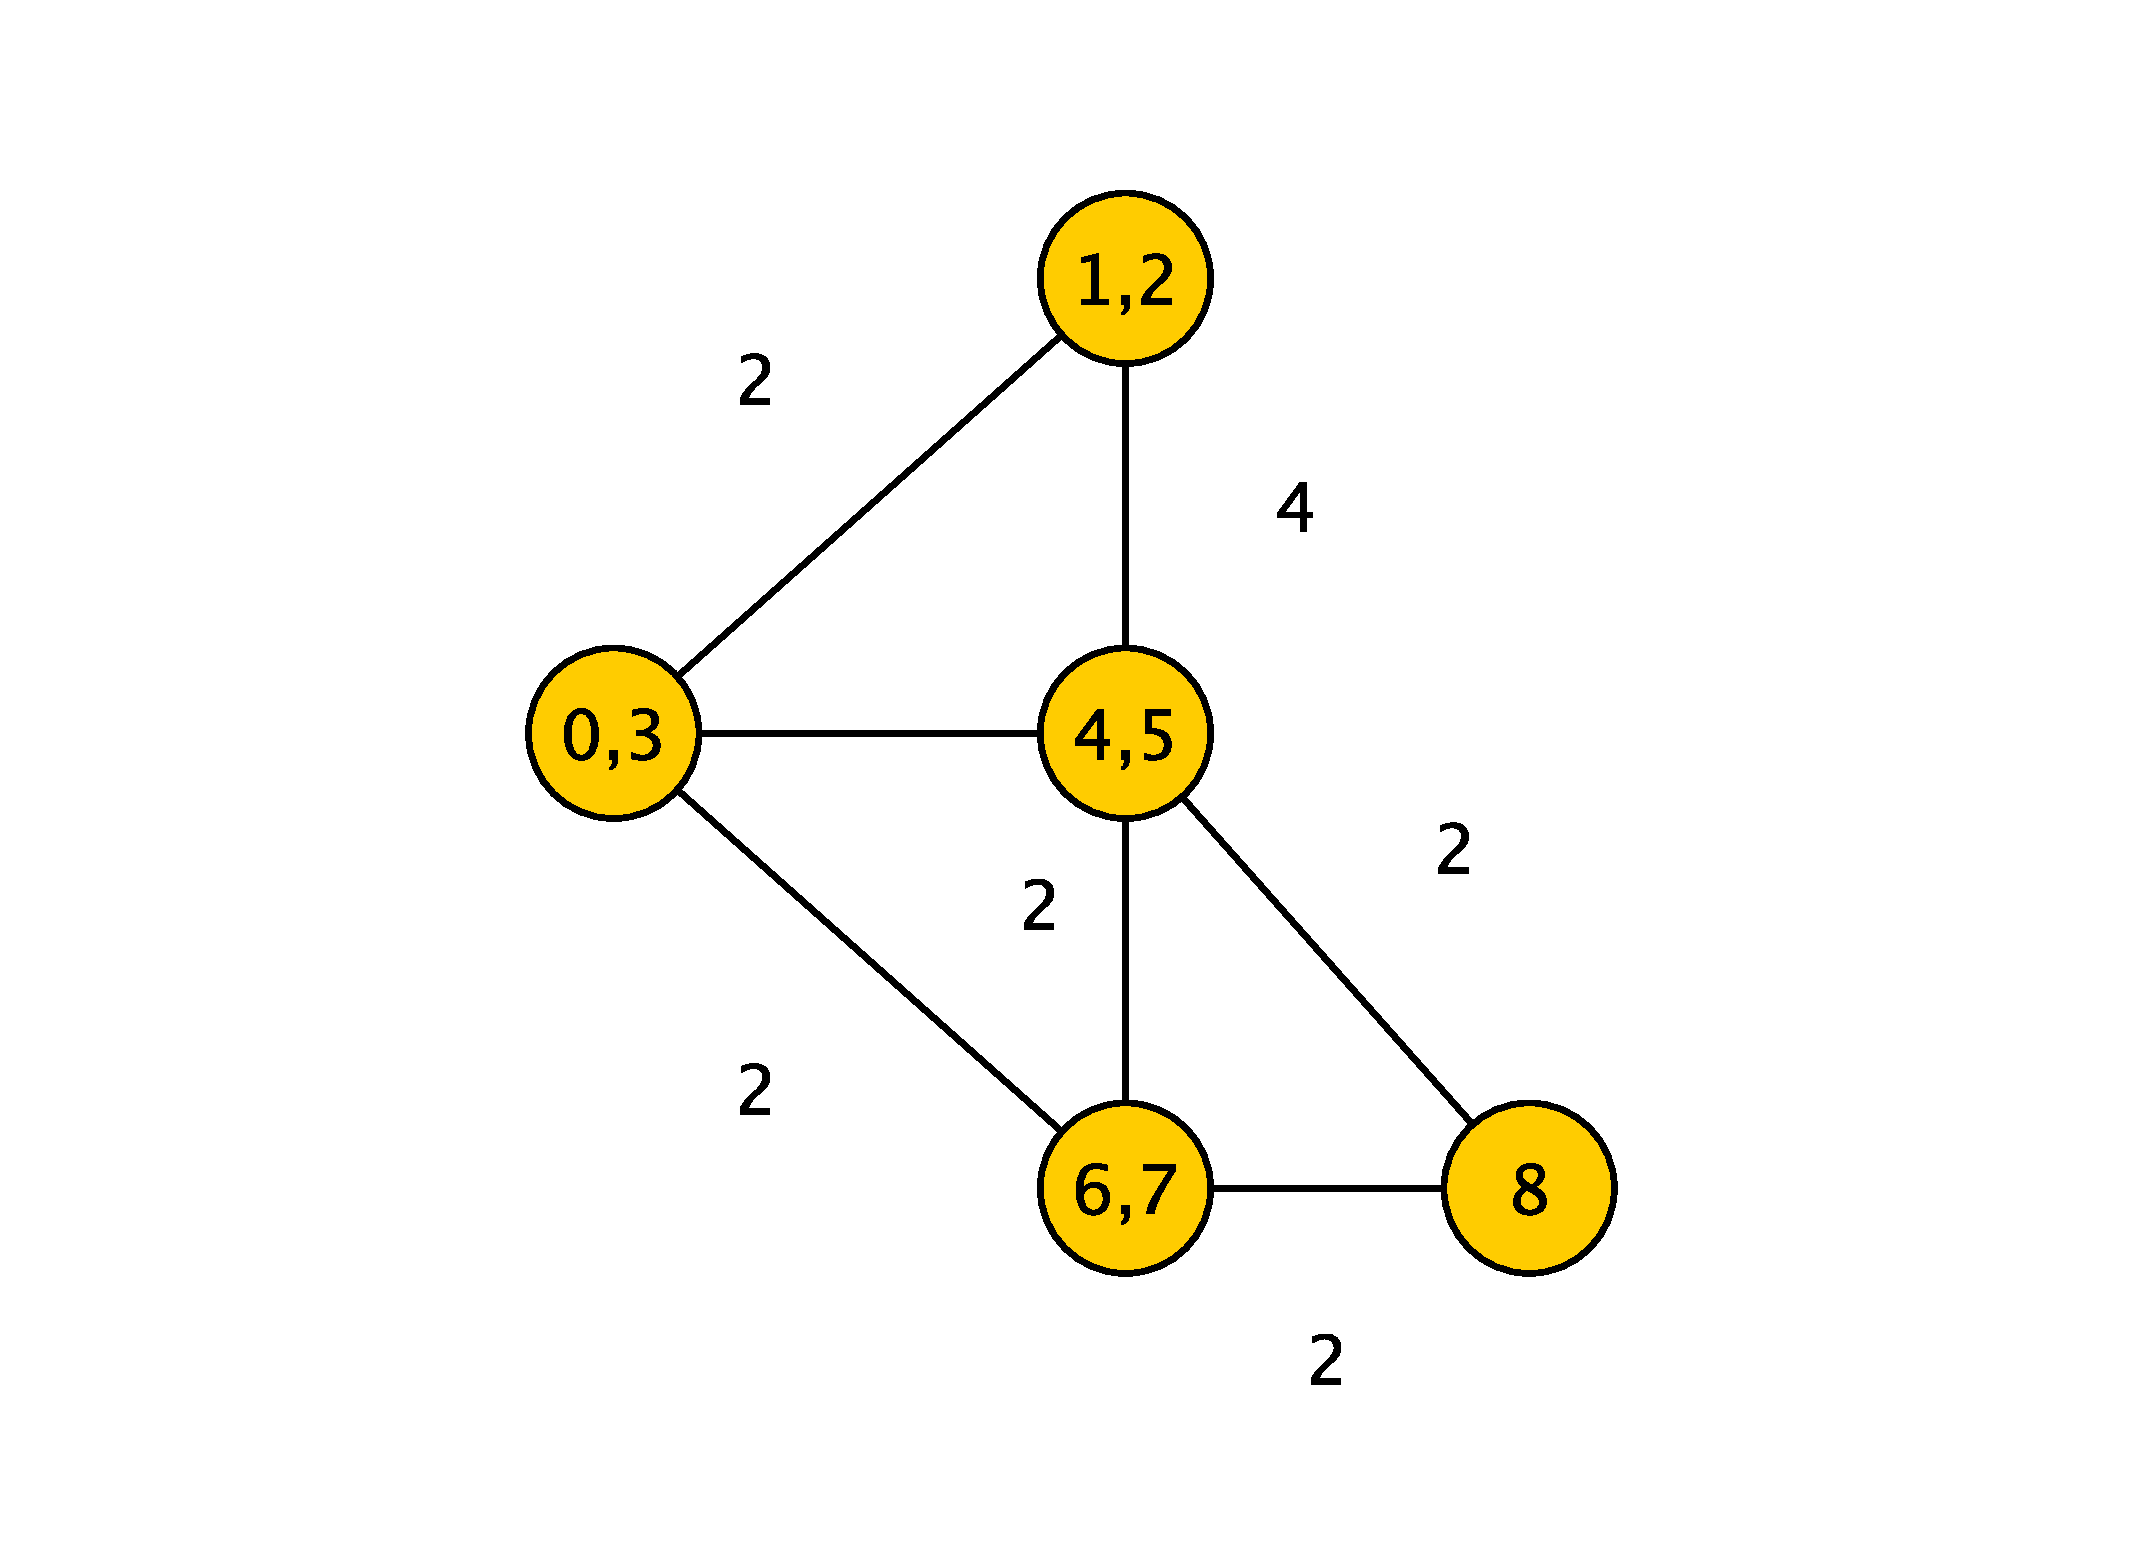
\includegraphics[width=\columnwidth]{img/coarsening2.eps}
    \caption{Coarsened graph}
    \label{img:coarse_graph}
  \end{figure}
\end{center}

Figure \ref{img:part_graph} displays the partitioned graph, this is the next step in the algorithm. To do this, a Greedy Graph Growing (GGGP) algorithm is used.\cite{Karypis:1998:FHQ:305219.305248} The goal of this phase, is to compute a high quality bisection (e.g., small edge-cut) of the coarsened graph such that each part contains roughly half of the vertices and edges of the original graph.
\begin{center}
  \begin{figure}[htb]
    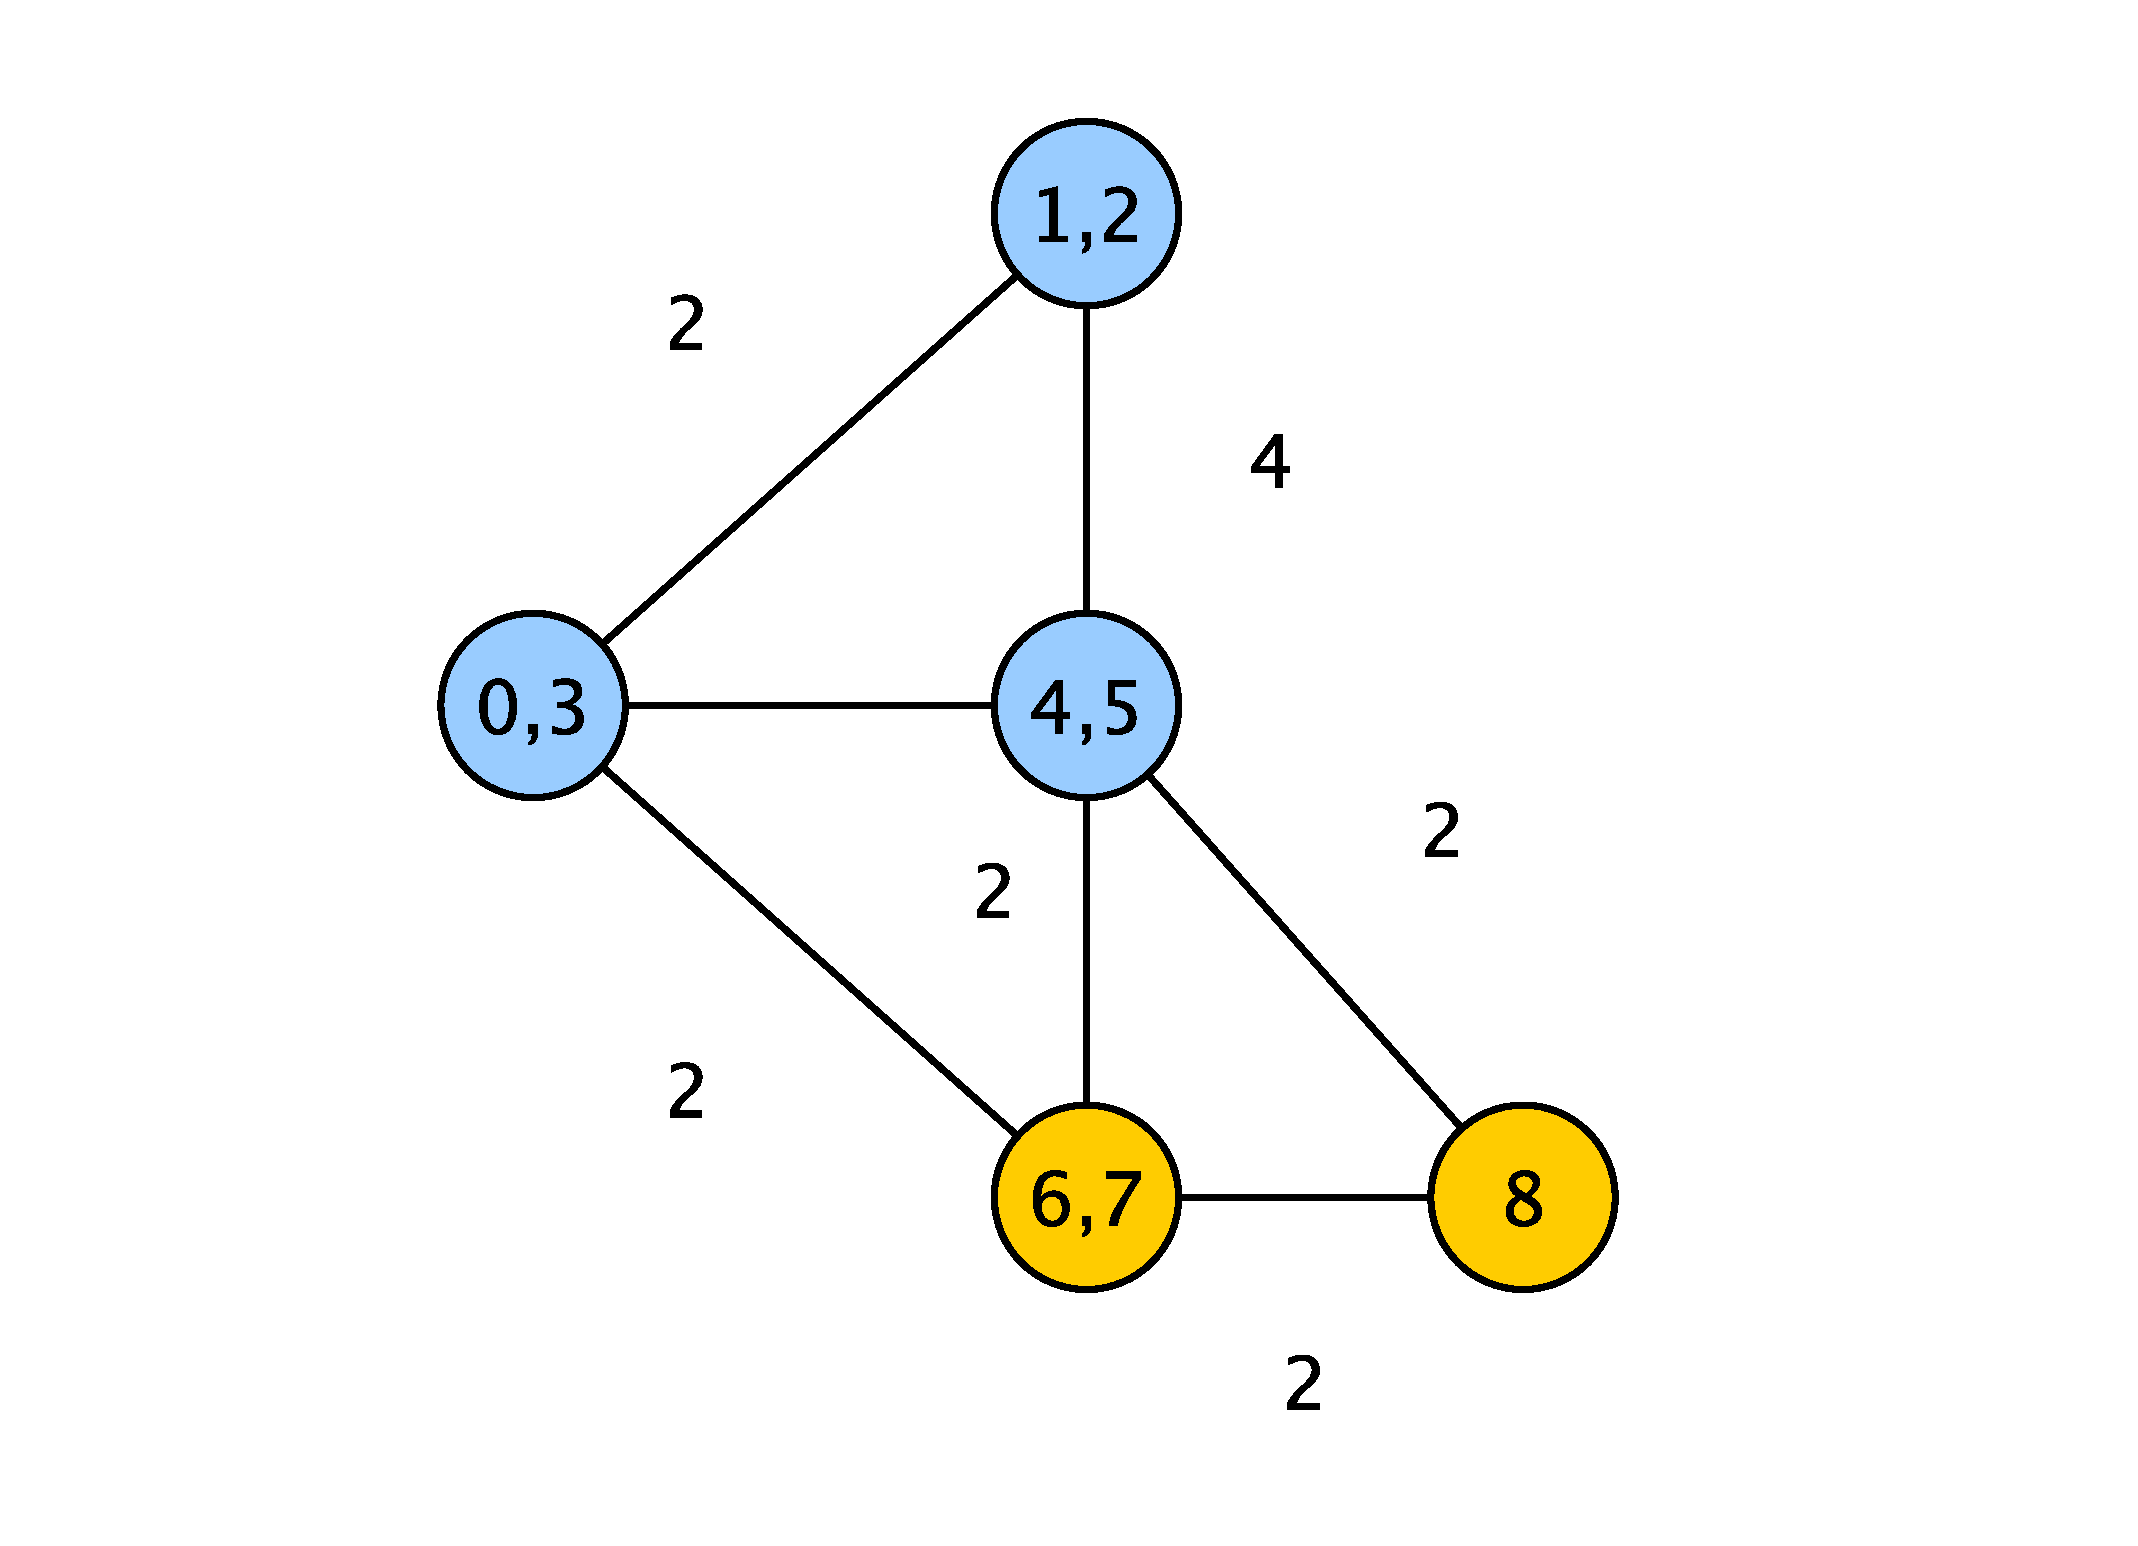
\includegraphics[width=\columnwidth]{img/partition.eps}
    \caption{Partitioned graph}
    \label{img:part_graph}
  \end{figure}
\end{center}

Figure \ref{img:refined_graph} shows the results of the refinement phase. During this stage, the partition of the coarser graph is projected back to the original graph by going through the graphs.\cite{Karypis:1998:FHQ:305219.305248}
Once again, the goal here, is to minimize the edge-cut, however, a good balance in the number of vertices assigned to each partition is also very important. Hence, in this final phase, some algorithms use special heuristics to further improve on the balancing achieved.
\begin{center}
  \begin{figure}[htb]
    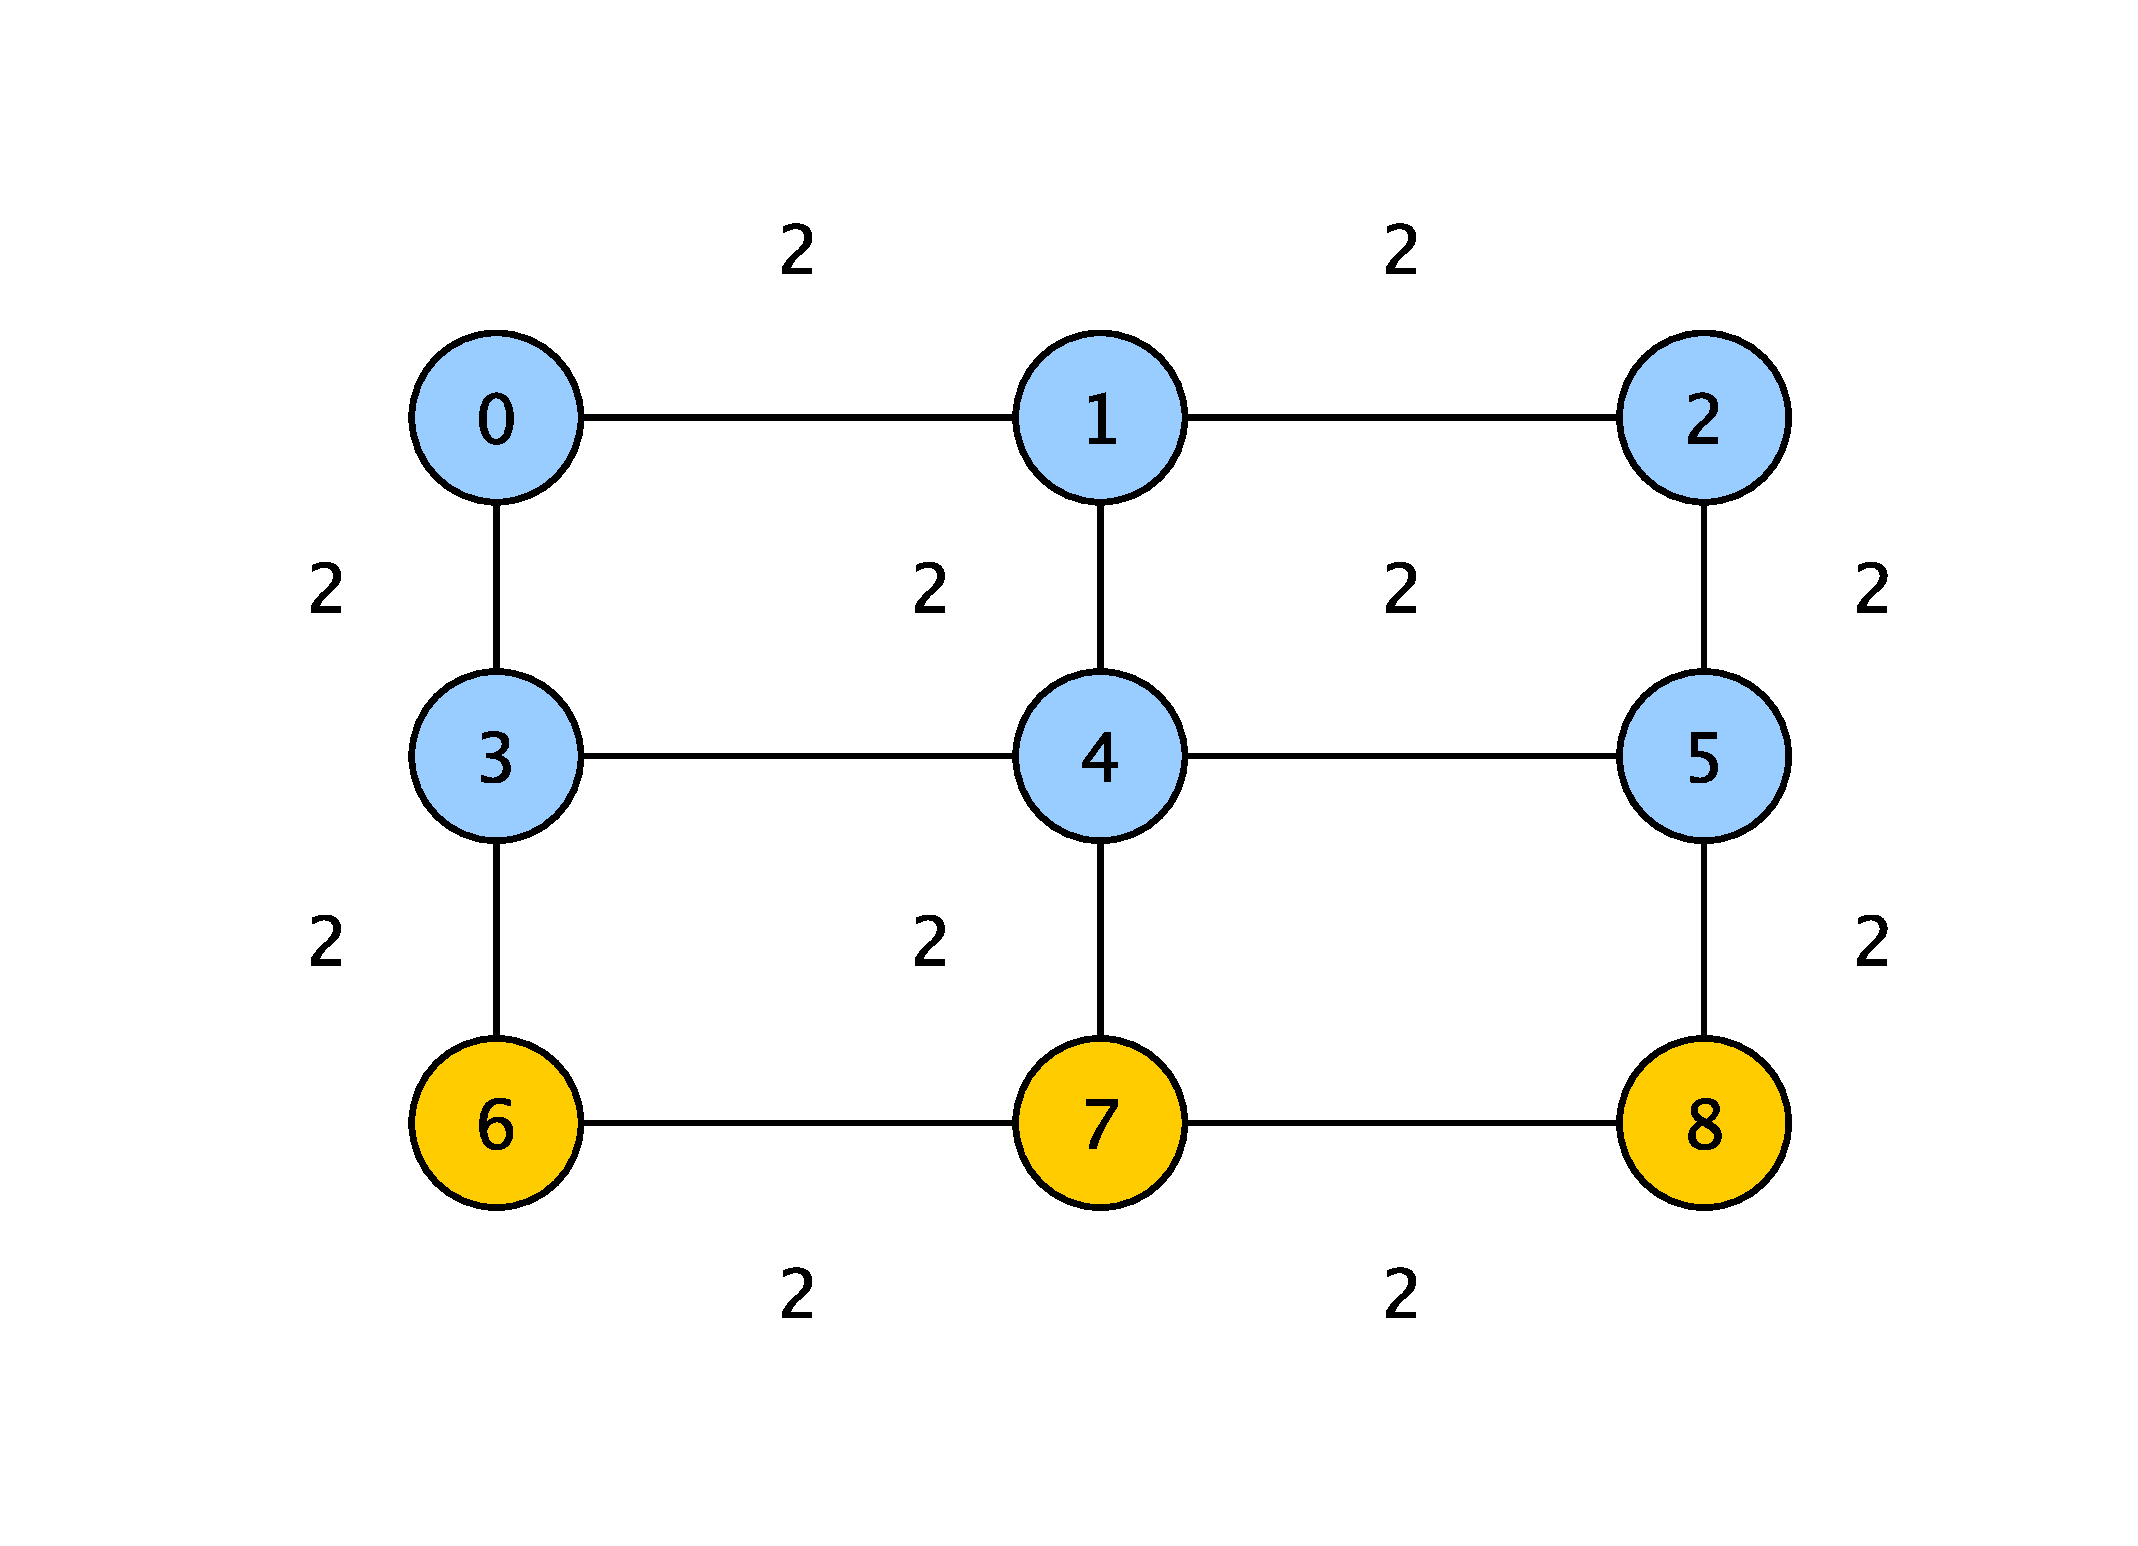
\includegraphics[width=\columnwidth]{img/refinement.eps}
    \caption{Refined graph}
    \label{img:refined_graph} 
  \end{figure}
\end{center}


%-----------------------------------------------------------------------------
% System characteristics
%-----------------------------------------------------------------------------

\section{System characteristics}
\label{sec:sys_char}
For the purpose of comparing the different applications, measurements
were performed in Stampede's co-processors. The co-processors are the
new Intel Xeon Phi with 61 cores. Its characteristics are presented in
the following table.

\begin{table}[H]
\centering
\footnotesize
\begin{tabular}{| c | c |}\hline
Manufacturer & Intel\\ \hline
Model & Xeon Phi SE10P\\ \hline
$\mu$Arch & Many Integrated Cores - MIC\\ \hline
Clock freq & 1.1 GHz\\ \hline
\#CPUs (sockets) & 1 \\ \hline
\#Cores/CPU & 61\\ \hline
\#Thread/Core & 4\\ \hline
L1 cache size/core & 32KB\\ \hline
L2 cache size/core & 512 KB\\ \hline
Main Memory/CPU & 8 GB\\ \hline
Vector width & 512 bits\\ \hline
\end{tabular}
\caption{Intel Xeon Phi}
\label{fig:mic}
\end{table}

Each core has support for 4 hyperthreads that shares 512 KB of the
second cache level. Thus, the total amount of second cache level is more
than 30 MB for the entire co-processor. The more powerful feature of MIC
is a vector unit of 512 bits for each core allowing the execution of 8
double precision or 16 single precision operations in parallel.
Globally, the floating peak performance of the Xeon Phi is given by:

\begin{itemize}
\item 16 (SP SIMD) x 2 (FMA) x 1.1 (GHZ) x 60 (\# cores) = 2112
  GFLOPS/sec for single precision arithmetic 
\item 8 (DP SIMD) x 2 (FMA) x 1.1 (GHZ) x 60 (\# cores) = 1056
  GFLOPS/sec for double precision arithmetic 
\end{itemize}

Each unit has support for fused multiply add operations, and together
with the vector units, Xeon Phi achieves theoretical peak performance of
more than 1 teraflop.

As can be seen, the Intel Xeon Phi only has 8 GB of memory, thereby
limiting large input graphs to run with GMetis. Therefore, all
measurements were done using the USA-W road-map as input, which is the
largest graph that still fits in memory. This graph contains 6262104
nodes and 15248146 edges.

Apart from the characteristics showed in table~\ref{fig:mic}, there are
others that should be mentioned. Image~\ref{img:phi_arch} shows a Xeon
Phi core were We can see its 4 hardware threads. Each core contains a
in-order dual pipeline which can issue two instructions from the same
hardware thread per clock cycle. However, the front-end of the pipeline
does not issue instructions from the same hardware thread in consecutive
cycles.\cite{Cepeda:PhiPerformance}

This means that if there is only one thread running on a core, for
instance T0, this threads may have two instruction issued on the first
clock cycle, but none on the second cycle. Thus, the maximum issue rate
is only attainable with at least 2 threads per core, so that in each
cycle, two instructions may be issued. Generally, the other two threads
have the purpose of hiding pipeline stalls due to memory latency so that
the maximum issue rate may be attainable.

Also, it should be noted that the fact that the pipeline issue
instructions in-order increases memory related problems. For instance,
when there is a stall on a hardware thread, this thread needs to wait
for data to be fetched from memory, which means more than 100 cycles.
This situation happens every time, which means that only four threads
per core might no be sufficient to hide such possible latency.

\begin{center}
\begin{figure}[htb]
    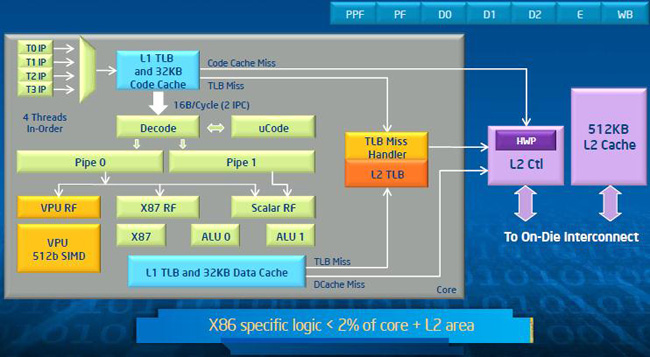
\includegraphics[width=\columnwidth]{img/phi_arch.jpg}
    \caption{Xeon Phi Coprocessor
    Core}\footnote{http://software.intel.com/en-us/articles/intel-xeon-phi-coprocessor-codename-knights-corner}
    \label{img:phi_arch}
\end{figure}
\end{center}


%-----------------------------------------------------------------------------
% Metis and Mt-metis
%-----------------------------------------------------------------------------

\section{Metis and Mt-metis}

%\section{Metis}

%The next plot shows the scalability of Mt-metis on Xeon Phi\footnote{All measurements were taken using version 0.1 of mt-metis.}. 
%Despite the large number of measurements taken, results shows spikes when running mt-metis with a certain number of partitions. We can see that
%mt-metis scales up to 28 threads, declining rapidly for more than 60 threads. 
%This is mainly due to the clustering and refinement stages, since, as we can see from the figure, the coarsening stage is relatively well behaved. 
%The behaviour of the refinement phase is somewhat to be expected, since, with the higher number of threads, as conflicts arise, it is expected for its running time to go up.
%The problem here, is the Partitioning (Clustering) phase, since its behaviour in unpredictable as the number of threads go beyond 60. We believe the explanation for this behaviour lies the Xeon Phi's architecture, since, as explained above, the maximum issue rate is 2. Combining this with a higher number of threads, the amount of stalls and ensuing context switches is expected to go up. This can be especially bad if the application has a lot of memory random memory accesses, which is the case.  


\label{sec:metis}
To compare both applications, their runtime and edgecut, we did some
scalability measurements. We measured metis time on one core of Xeon Phi, 
and mt-metis for all possible number of threads.

The next figure shows the scalability of Mt-metis on Xeon
Phi\footnote{All measurements were taken with the version 5.1.0 and 0.1
of Metis and Mt-metis respectively}. Despite
the large number of measurements taken, results shows spikes when
running mt-metis with a certain number of partitions. The figure also
shows speedups relative to the runtime of one thread of mt-metis. We can
see that mt-metis scales up to 28 threads, declining rapidly for more
than 60 threads. The runtime from 29 up to 59 varies radically. For more
than 60 threads, the increasing runtime is mostly due to the clustering
and refinement stages. A similar situation happens with gmetis, but as
we will see in~\ref{sec:gmetis}, the costly phase with a high number of
threads is different. 
We do not understand perfectly the reason why this happens. With one or
few number of threads, the phase that takes more time is Coarsening,
followed by Refinement and then Clustering/Partition which is more or
less what is expected to happen. But with a high number of threads, this
situation changes with the phase that was taking more time before now
being the one that takes less time. As we focused only on GMetis, we are
not able to tell why this happens.
This example is for 128 partitions, but we did
measurements for different number of partitions, such as 16 and 1024,
and all of them shows a similar behavior, reason why only the image
with 128 partition was presented.

\begin{center}
\begin{figure}[htb]
    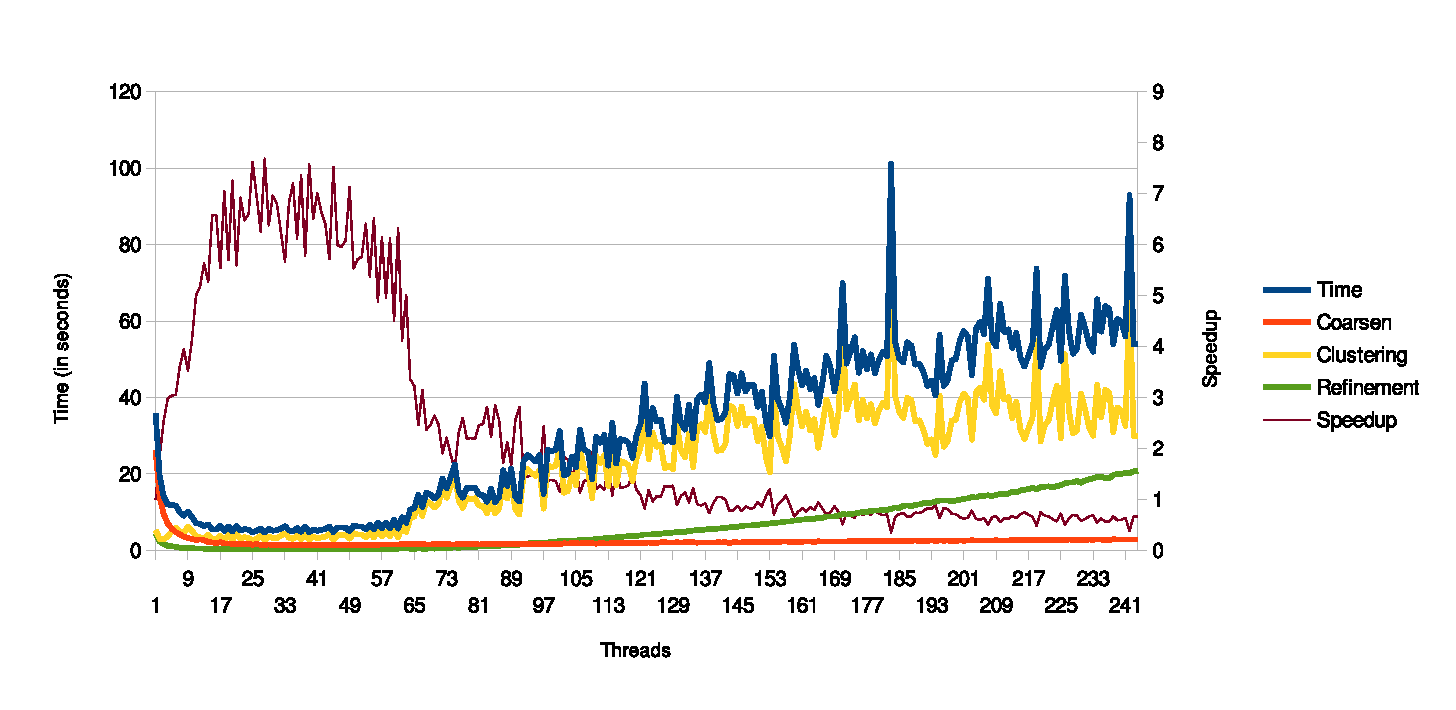
\includegraphics[width=\columnwidth]{img/mtmetis128.eps}
    \caption{Mt-metis - 128 partitions}
    \label{img:mtmetis128}
\end{figure}
\end{center}


%-----------------------------------------------------------------------------
% GMetis and Galois Framework
%-----------------------------------------------------------------------------

\section{GMetis} 
\label{sec:gmetis}
The measurement for GMetis was done in the same way as mt-metis, that
is, for all possible number of threads. Figure~\ref{gmetis128} shows the
scalability of gmetis on Xeon Phi for 128 partitions. We can see a
similar behavior with mt-metis, with the differences that gmetis scales
for a higher number of threads, it does not have a irregular behavior
and the performance declines less suddenly.

\begin{center}
\begin{figure}[htb]
    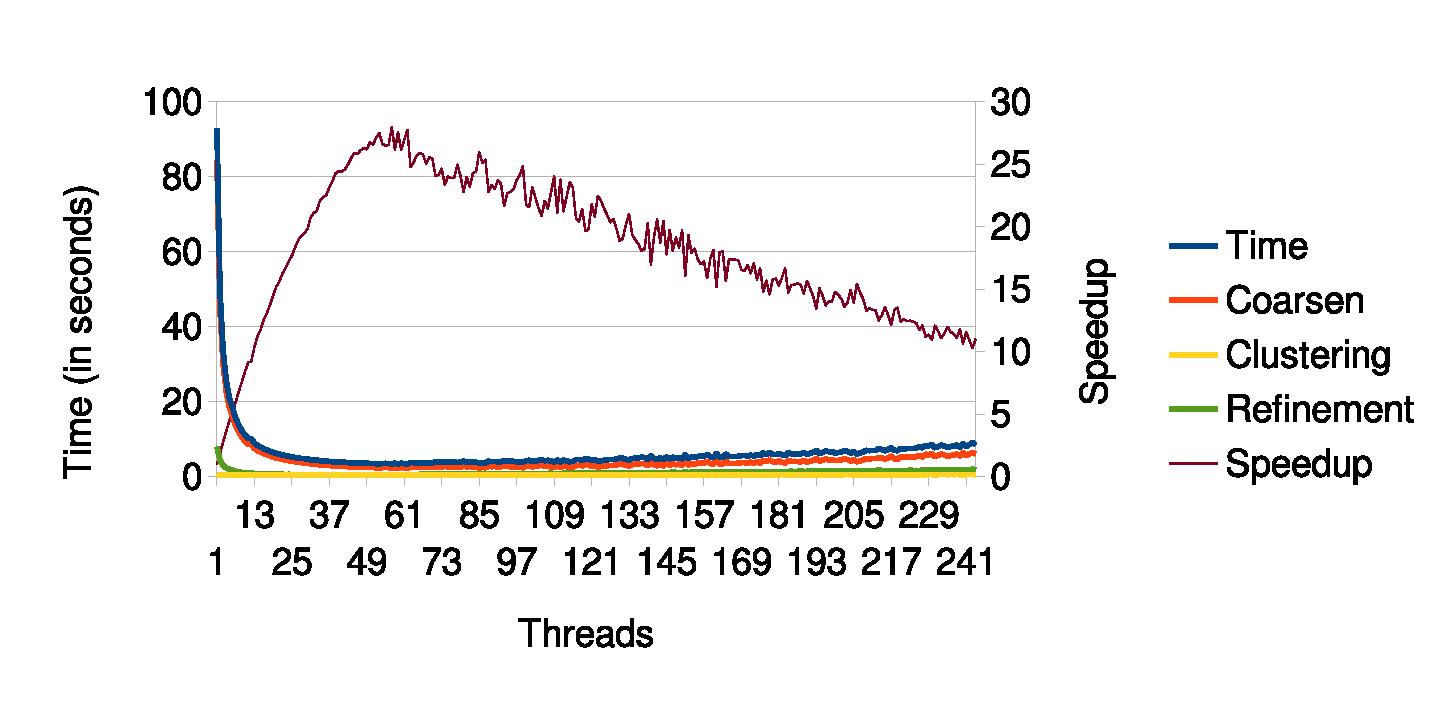
\includegraphics[width=\columnwidth]{img/gmetis128.eps}
    \caption{GMetis - 128 partitions}
    \label{gmetis128}
\end{figure}
\end{center}

As with mt-metis, the speedup presented in the figure is relative to the
runtime of one thread of gmetis when ran on one core of Xeon Phi. Gmetis
scales to 70 threads were it attains its maximum peak performance, and
decreases linearly with more threads. With more than 70 threads, the
global time is more affected by the Coarsening phase. This behavior is
different from mt-metis were the Clustering phase was the heavier.
Although gmetis scales better than mt-metis, the latter proves to be
really fast for one or few threads as opposed to the former. For
instance, if Xeon Phi only provided 28 threads, mt-metis would
surely run faster than gmetis.

%-----------------------------------------------------------------------------
% Enhancements
%-----------------------------------------------------------------------------
\subsection{Enhancements}
\label{sec:enhan}
Throughout this month, we did some modifications to improve
\textit{GMetis}' performance. We started by experimenting how the
package mapping is done internally by the \textit{Galois} framework.

\textit{Galois} has support for \textit{NUMA} systems, thus, this means
that it takes advantage of different sockets (packets in Galois
terminology) simultaneously.

Before an application starts running, \textit{Galois} parses the cpuinfo
file located in "/proc/cpuinfo" to create its mapping, which means that
each socket corresponds to a package, or rather, all the cores in a
socket belong to the same package.  This means that \textit{Galois} was
assigning a package to the entire MIC co-processor, since it has 60
usable cores in the same "package".

This is especially bad, since the \textit{Galois} framework uses a sort
of work stealing mechanism inside each package, to provide good load
balance. It works by assigning a master thread in each package, then
each thread inside a package can steal work from another inside the same
package. In case of aborts, the work is pushed to a stack in the master
thread, if it aborts when that master thread pops from the stack, then
the work is pushed in another packet's stack. In the MIC, since there is
only one packet, this means that all 244 threads were stealing work from
each other. Hence, worst case scenario, the code is run serially. 

Also, it should be noted that, since \textit{Galois} was not prepared to
deal with a processor that supports more than two-way hyperthreading,
when using different thread values, some processor cores could have four
threads running, while others only one (default mapping).

We changed that, by assigning each hyperthread to its respective core id
(which would make a packet).  Another reason for this change is so that
the mapping could be the most balanced possible (load balanced
mapping)\footnote{Although the Xeon Phi contains 61 cores, it should be
  noted that the operating system also needs to run. Therefore, only 60
cores may be available for computations tasks. With 61, an application
can be affected by the operating system noise}, for instance, when
running the application with 121 threads, with the default mapping, the
first 20 cores will run with four threads while the others will only run
with one thread. With the load balance mapping, only the last core will
run one thread, while the others will run 2 threads. However, this did
not achieve any considerable improvements. We also tried assigning each
thread to a packet in a round-robin fashion (dense package mapping), but
that proved to be ineffective as well (as expected).

To improve gmetis performance, we profiled the application.
Unfortunately, Intel VTune only has support for Stampede's hosts, and
not for the co-processor. Although, Intel states that profiling and
improving an application on the host gives similar improvements on MIC,
profiling support for the MIC architecture on \textit{Stampede} would be
welcome, as there are key differences in the architectures.

Thereby, we profiled the application with the help of simple timers as
well as PAPI, and we found the most time consuming function, which is
\textit{findMatching}. This function iterates through the graph's nodes,
trying to match each node with one available neighbor.

This function is part of the \textit{Coarsening} phase, together with
the \textit{CreateCorseEdge}.
The coarsening phase as the objective of coarsening a graph so it can be
more easily partitioned. This is done mainly in two phases. The first,
findMatching, matches nodes that have not been matched yet, and creates
a "supernode" for each pair of matched nodes. The
\textit{CreateCorseEdge} creates the edges between "supernodes", merging
edges that are shared between the two nodes of the supernode and their
common neighbors. The merging operation implies the sum of the weights
of these shared edges.

There are different ways to match the graph's nodes. The ones used are
"Heavy Weight Match" and "Random Match". The first iterates through each
node and matches them with the neighbor whose shared edge has the most
weight. The second matches each node with the first neighbor node that
has not been matched yet. Nodes that cannot be matched with any other
node are not merged. Supernodes are created from these single nodes.

Previously, these two algorithms were used separately, i.e., only one of
them was used in the application. Using the two combined proved to be a
better solution, as the performance improved, and the edge-cut remained
the same. Random Match is used in the first two iterations of the
coarsening phase. This improved runtime because, RM computes faster, as
it does not need to iterate through all neighbors when there is a node
that has not been matched. The algorithm is used only on the first two
iterations because the graph is larger on these iterations, and using RM
instead of HEM on small graphs did not prove to be any faster and can
actually worsen edge-cut.

Has the timers and PAPI were not giving helpful information, we tried to
manually fetch some information based on a guess that findmatchting
would incur in many misses (mainly because of in-order pipeline). On
previous processors that did not contained out-of-order pipelines,
software prefetching was almost always useful. 
We prefetch neighbor nodes, as these were given by an array whose
indexes were also given by another array. In this type of situations,
prefetch is almost always impossible to happen. 
However, prefetching did result in improvements.
A deeper look into the assembly code generated by the gcc compiler 
showed that it does not introduce prefetch instructions (even when using
\_\_builtin\_prefetch). On the other hand, icc does some prefetch. The results,
however are quite similar to the gcc ones.

Finally, we also did some tests with different worklist schedulers provided by
Galois. AltChunkedLIFO was the fastest and it is actually the most
scalable one, which improved a little application's runtime.

%-----------------------------------------------------------------------------
% Final results
%-----------------------------------------------------------------------------

The following figure compares the runtime of each application. Metis was
executed in one of the Xeon Phi's core, while mt-metis and gmetis were
executed for each number of threads, for the three partitions number.
For those, the best execution time was chosen. The time of the
sequential metis is included to see how much speedup both mt-metis and
gmetis obtains for each partition number. We can see that for 16
partitions, mt-metis run faster than gmetis, achieving a total speedup
of 24x as opposed to the 17x of gmetis. For the other number of partitions,
gmetis is actually faster, achieving a total speedup of 17x and 11x for
128 and 1024 partitions respectively. For the three number of partitions, mt-metis
achieves its maximum performance with more or less 30 threads whereas
gmetis achieves it with 70 threads.

\begin{center}
\begin{figure}[htb]
    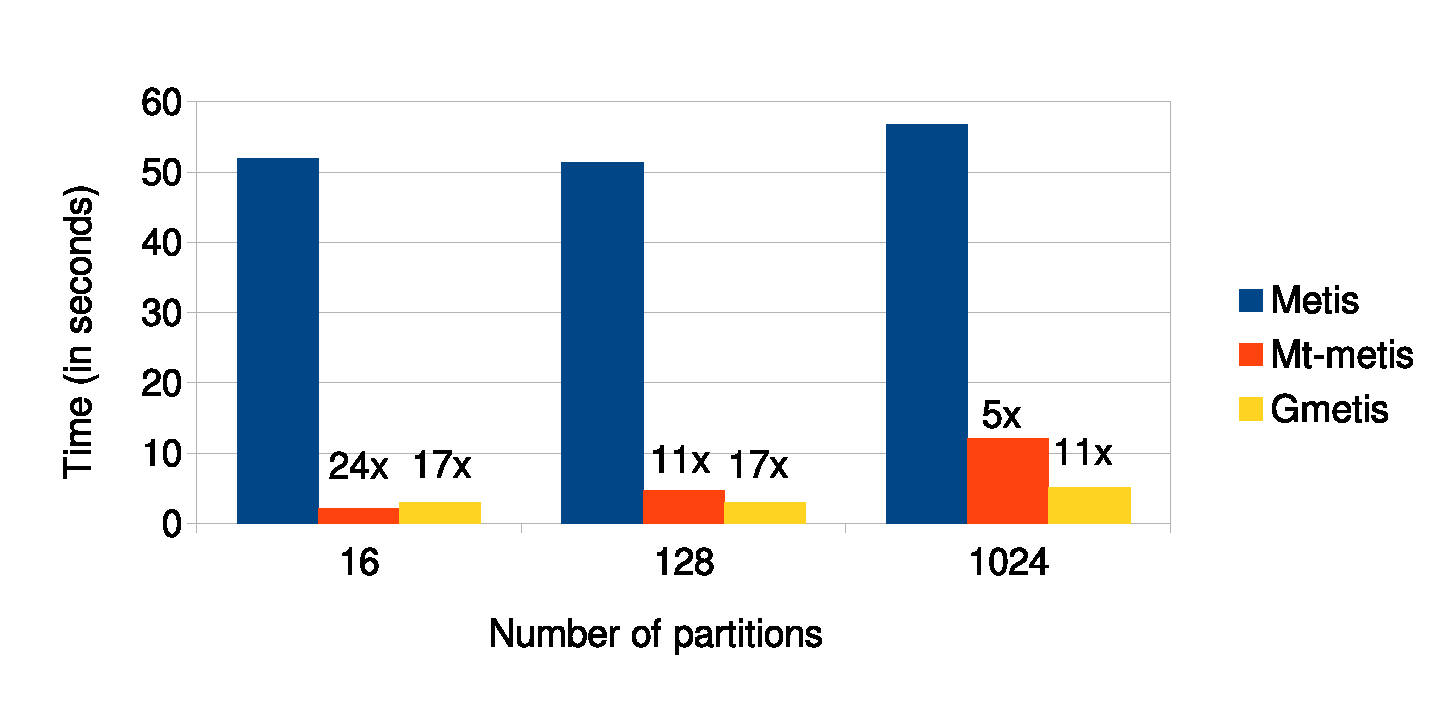
\includegraphics[width=\columnwidth]{img/comparison3.eps}
    \caption{Comparison}
    \label{img:comparison3}
\end{figure}
\end{center}

We made some extra measurements that allowed us to find that with 45-50
partitions, GMetis start to run faster than mt-metis.

%\begin{center}
%\begin{figure}[htb]
    %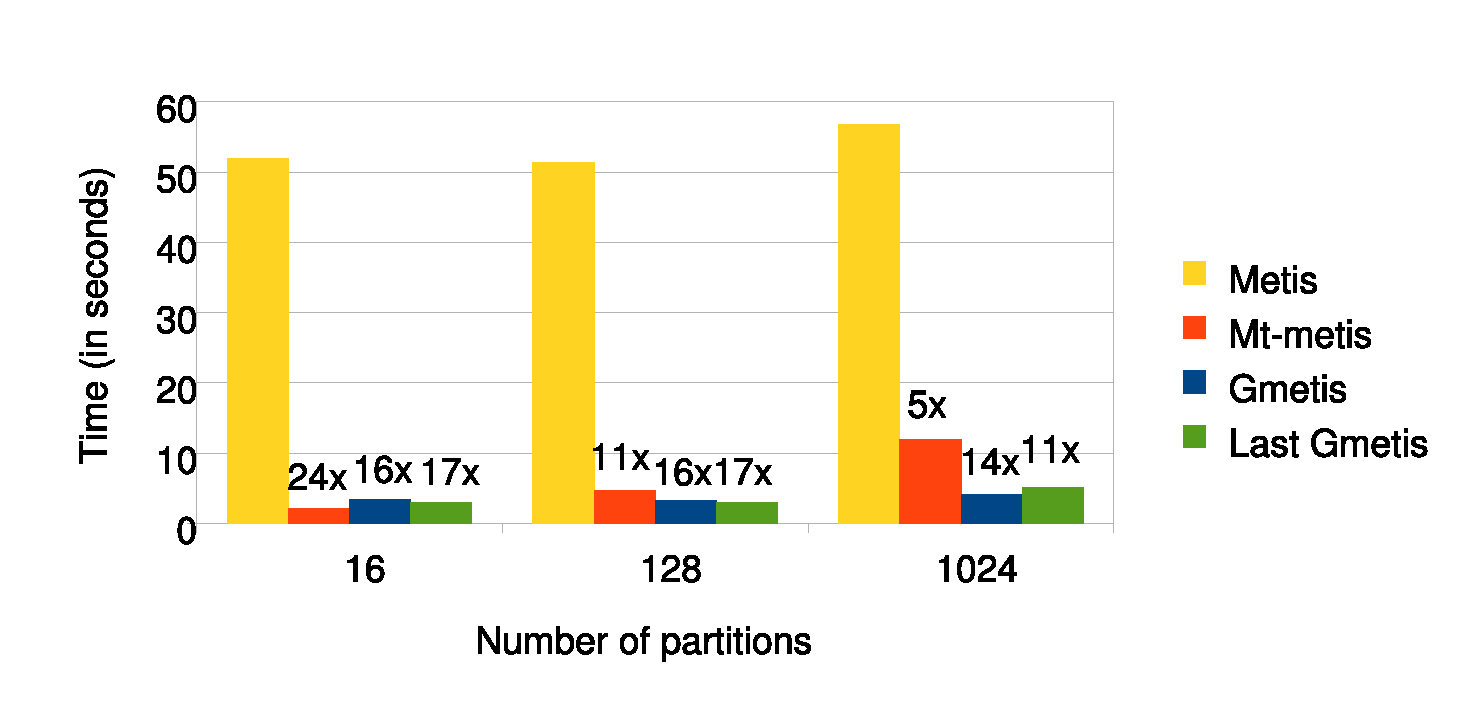
\includegraphics[width=\columnwidth]{img/comparison4.eps}
    %\caption{Comparison}
    %\label{img:comparison4}
%\end{figure}
%\end{center}

%TODO: Falar que o metis tenta obter partições o mais balanceadas
%possiveis na parte da introdução
As previously stated, the objective of \textit{Metis} is to partition a
graph in a way that the partitions are balanced and the edge-cut between
them is the smallest possible. For this last metric, GMetis performs
worse. According to the measurements made and that are showed on figure~\ref{img:edgecut},
\textit{GMetis} edge-cut is always more than two times higher than metis
and mt-metis. The openMP version of metis performs a little bit worse
than its original version.

\begin{center}
\begin{figure}[htb]
    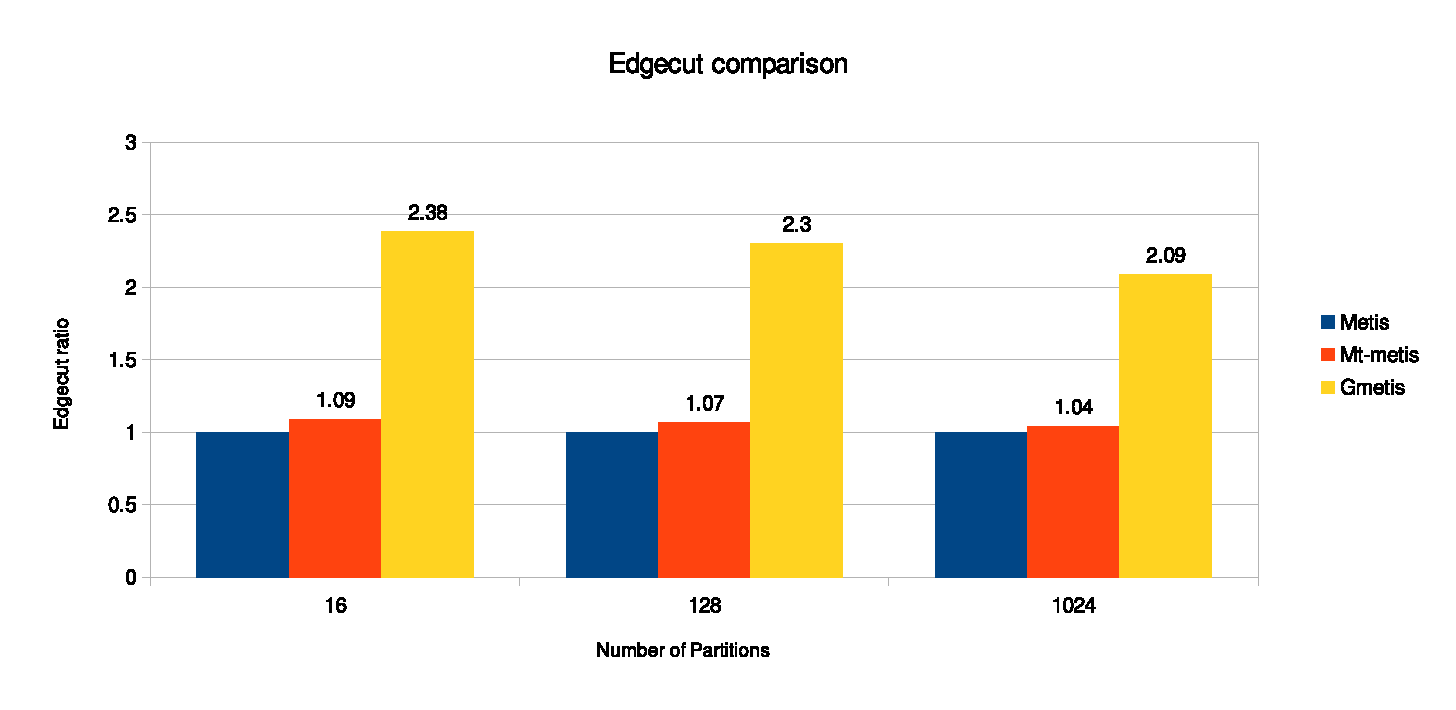
\includegraphics[width=\columnwidth]{img/edgecut.eps}
    \caption{Comparison}
    \label{img:edgecut}
\end{figure}
\end{center}


%-----------------------------------------------------------------------------
% Conclusion
%-----------------------------------------------------------------------------

\section{Conclusion}
\label{sec:conc}
Results showed that both \textit{Metis} and \textit{Mt-metis} have
better edge-cut than \textit{Gmetis} for all number of partitions tested. 
These two application also run faster than GMetis, for 16 partitions.
However, Gmetis's runtime is lower for a high number of partitions, i.e.
128 and 1024 partitions.

Further analysis showed that GMetis start to run faster than mt-metis
with more or less 45-50 partitions. However, both metis and mt-metis provides
better edgecut.
Although the difference of the edgecut between the applications may seem
high, it may be not relevant for an higher number of partitions if
GMetis computes the partitions much faster than mt-metis. For real
applications that uses the metis algorithm, the time consumed
calculating the partitions may be more important than a difference of
two time for the edgecut.

%-----------------------------------------------------------------------------
% Bibliography
%-----------------------------------------------------------------------------

\bibliographystyle{plain}
\bibliography{references}


\end{document}
